\documentclass[10pt,a4paper]{article}
\renewcommand{\baselinestretch}{1.0}
\usepackage{cite}
\usepackage[dvips]{graphicx}
\usepackage{psfrag}
\usepackage{color}
\usepackage[cmex10]{amsmath}
\usepackage{amsfonts}
\usepackage[font=footnotesize, captionskip=10pt]{subfig}
\usepackage{tikz}
\usepackage{flushend}
\usepackage{times}
\usepackage[margin=1.5cm]{geometry}
\usepackage[slovak]{babel}
\usepackage[utf8]{inputenc}
\usepackage[T1]{fontenc}
\usepackage[]{algorithm2e}

\usepackage{graphicx}
\usepackage{subfig}

\pagestyle{empty}

\hyphenation{net-works}
\newtheorem{remark}{Remark}

\begin{document}

\title{Effect of unsupervised pretraining in deep reinforcement learning}
\author{Michal Chovanec, michal.nand@gmail.com \\
Peter Šarafín, peter.sarafin@gmail.com}
\date{}
\maketitle
\thispagestyle{empty}

%\noindent$^1$\ affiliation\\
%\noindent$^2$\ affiliation\\

\noindent {\bf Keywords:}{reinforcement learning, function approximation, SARSA, Q-learning, neural network, unsupervised training}

\noindent {\bf Abstract:}

Článok sa zaoberá vplyvom unsupervised learning na celkový priebeh reinforcement learning tréningu.
Ako aproximátor funkcie ohodnotení je zvolená hlboká neurónová sieť.
Overovali sme hypotézu, že unsupervised predtrénovaná sieť sa v režime supervised učí
rýchlejšie. Zároveň sa ale očakáva, že obe siete po dostatočnom počte iterácií učenia
poskytnú rovnaké výsledky.
Dalšia testovaná hypotéza je vplyv riedkosti váh na kvalitu výsledku - dnešné
technické prostriedky sú navrhnuté na výpočty hustých sieti {\bf TODO citovat}, v budúcnosti, by
však hárdverovo akcelerované riedke siete mohli priniest výrazný nárast výkonu {\bf TODO citovat}.
Dôležité je preto overiť vplyv riedkych váh na výsledok.

\section{Introduction}

Reinforcement learning umožuje tránovať agenta v Markovovich rozhodovacích procesov tak
aby maximalizoval dosiahnutú odmenu.
Tradične sú používané algoritmy Q-learning {\bf TODO citovat} a SARSA {\bf TODO citovat}.
V tomto článku je použítý algoritmus SARSA, popísaný ako

\begin{equation}
  \label{eq:rl_sarsa_learning}
  Q'(s, a) = (1-\alpha)Q(s, a) + \alpha \Big(R(s, a) + \gamma Q(s', a') \Big)
\end{equation}

kde \\
$Q(s, a)$ je ohodnotenie akcie $a$ v stave $s$, \\
$R(s, a)$ je odmena za vykonanie akcie $a$ v stave $s$, \\
$\alpha \in (0, 1)$ je rýchlosť učenia, \\
$\gamma \in \langle 0, 1 \rangle$ je discount factor, \\
a $Q'(s, a)$ je nová hodnota ohodnotenia. \\

Pre malé stavové priestory (väčšinou len učebnicové príklady) je možné použiť tabuľku na
uloženie $Q$ hodnôt.
Pre veľké stavové priestory - je nevyhnutná aproximácia $Q$ hodnôt.
Často používané sú lineárna kombinácia bázových funkcií {\bf TODO citovat}
alebo dopredná neurónová sieť {\bf TODO citovat}.
\\
Rekurentná povaha rovnice \ref{eq:rl_sarsa_learning} spôsobuje že učiaci proces je
neefektívny a pomalý.
\\
Naša myšlienka je zameraná na unsupervised predtrénovanie siete a až po tom
trénovať použitím SARSA algoritmu.

\newpage
\section{Popis experimentu}

Agent bol umiestnený do hry znázornenej na obrázku \ref{img:Testing arcade game}.
Úlohou je preskakovať a podliezať červené prekážky, agent má teda na výber dve akcie.
Prekážky sa generujú náhodne, a postup je sprava do ľava. Za úspešné vyhnutie sa kolízií
získa agent odmenu $+0.3$, za neúspech $-1.0$. Toto je nevyváženie je dôležité,
pre kvalitatívne overenie algoritmu, aby náhodnými akciami nikdy nedosiahol kladné
skóre.
\\
Stav sú jednotlivé políčka hry, v tomto prípade 5x19 (95 prvkový vektor).
Hodnota $0$ znamená voľné (biela), hodnota $1$ reprezentuje agenta (zelená),
a hodnota $-1$ je zvolená pre prekážku (červená).

\begin{figure}[!h]
  \centering
  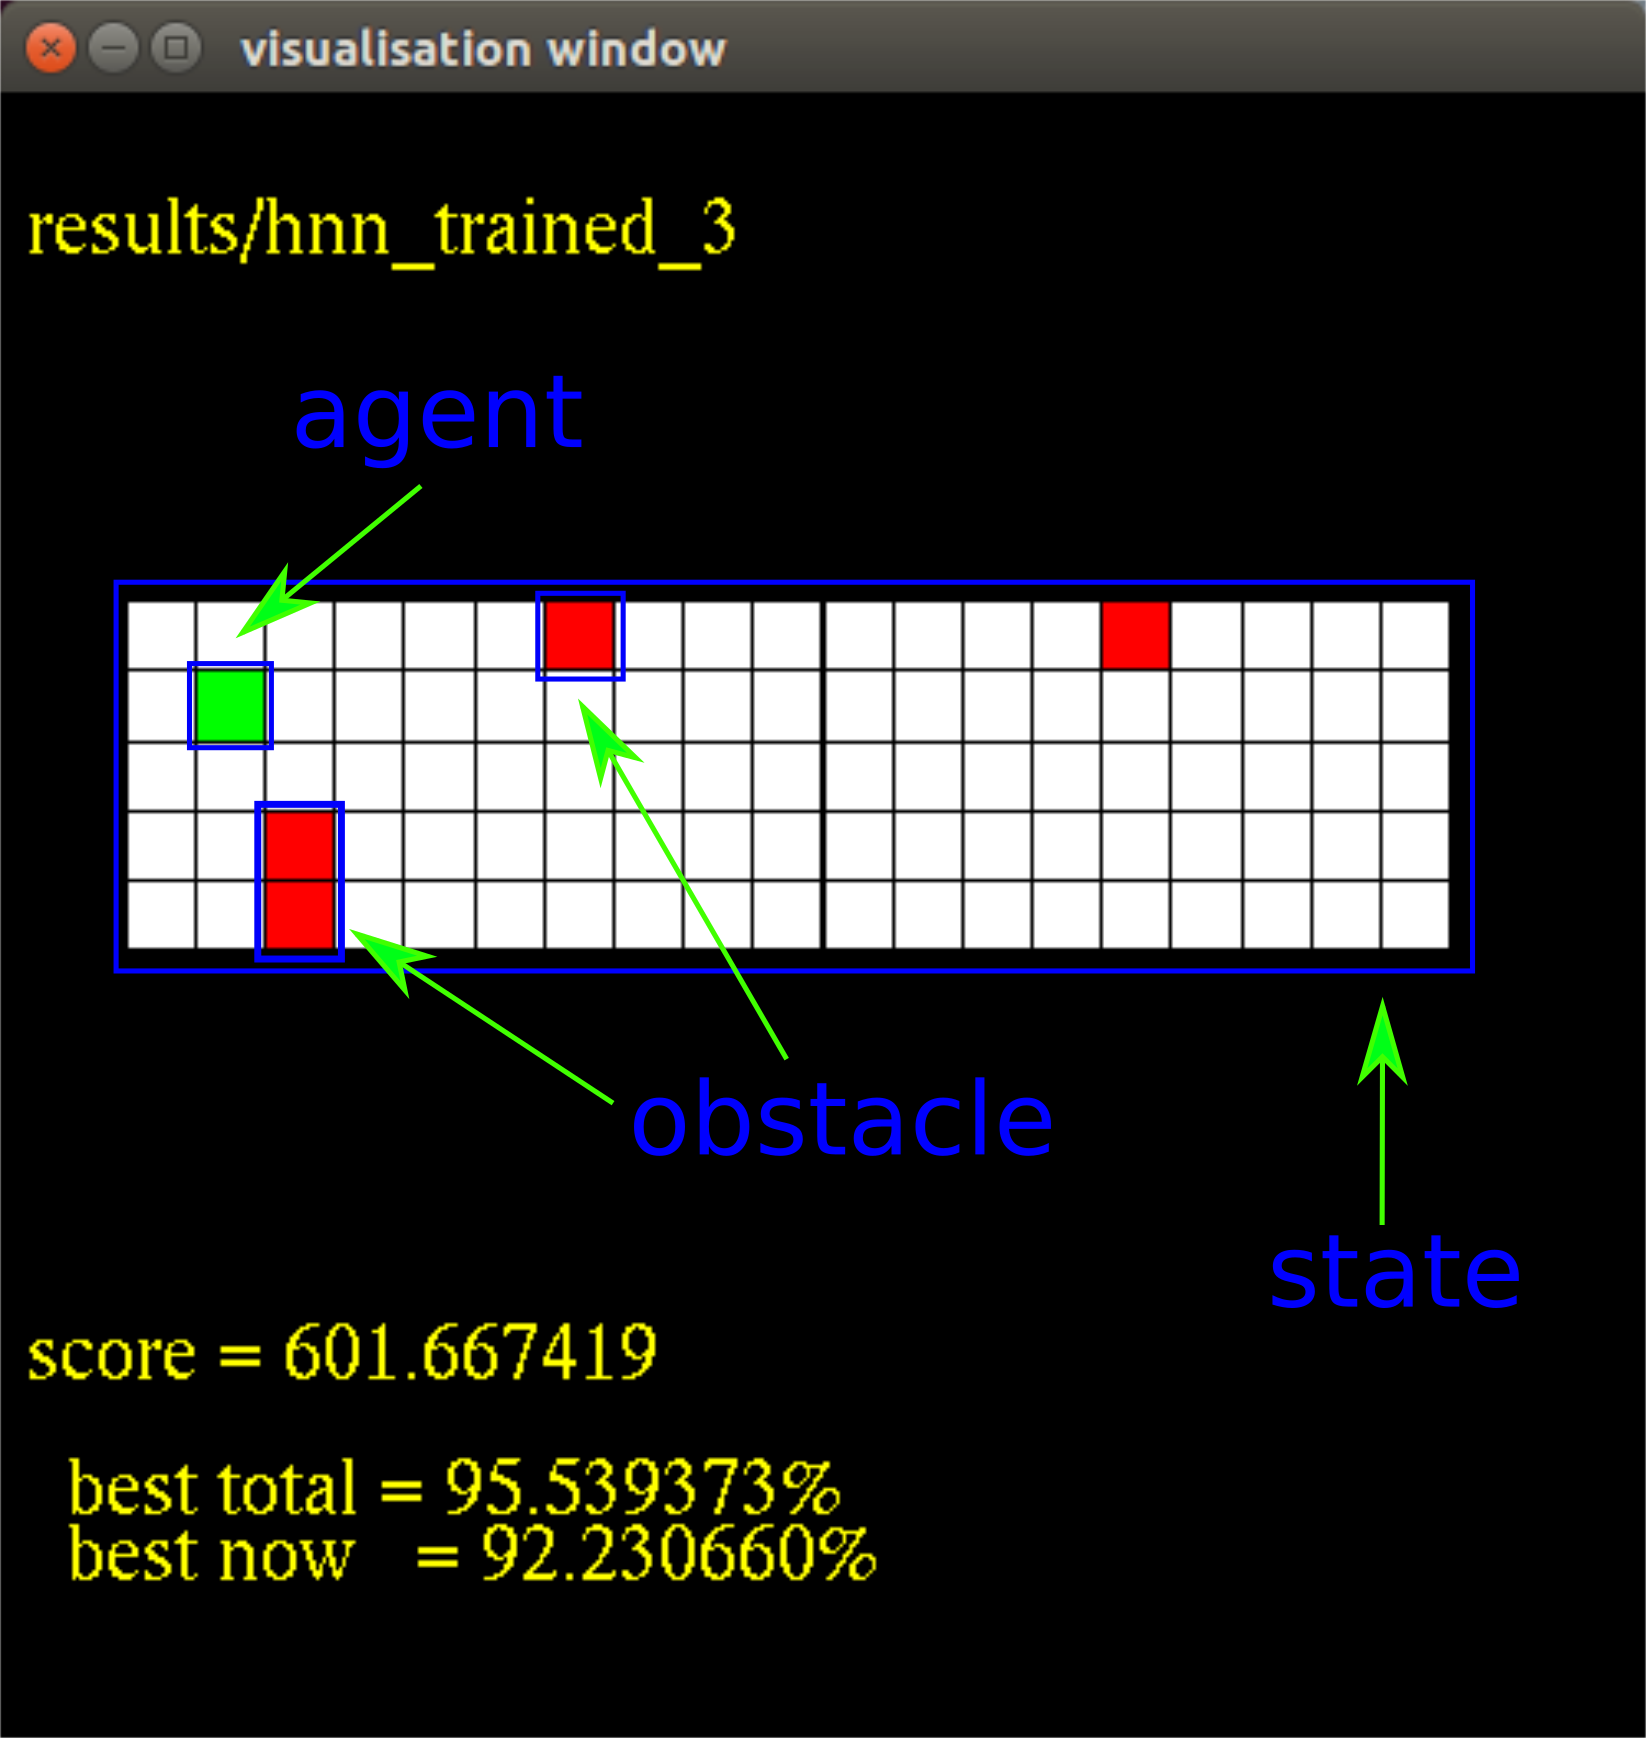
\includegraphics[scale=0.4]{../../diagrams/arcade_rl_game_desc.png}
  \caption{Testing arcade game}
  \label{img:Testing arcade game}
\end{figure}

V hre sa sleduje niekoľko veličín.
Celkové skóre je dané súčtom jednotlivých odmien. Ďalej sme zaviedli
ďalšie dve pomocné veličiny - best\_total a best\_now. \\
Veličina best\_total ukazuje, koľko percent času volil agent správnu akciu - vyhol sa kolízií,
od začiatku behu hry \footnote{Orientačne sme zistili, že ľudský hráč je schopný hrať v intervale od 91\% do 93\%.}. \\
Veličina best\_now ukazuje ukazuje voľbu najlepšej akcie len za posledné obdobie - je použitý
priemer s exponenciálnym zabúdaním.


\subsection{Topológia siete}

Pre porovnanie sme zvolili dve siete. Vstupom je stav hry 5x19 (95 prvkový vektor),
výstupom je hodnota $Q(s)$ pre každú akciu - skočit / neskočiť.
\\
Prvá siet je dopredná sieť (FNN) s dvoma skrytými vrstvami, topológia je na obrázku \ref{img:Supervised network architecture}.
Čísla nad vrstvami sú počty neurónov.
Skryté vrstvy majú aktivačnú funkciu ReLU, výstupná vrstva lineárnu aktivačnú funkciu.

\begin{figure}[!h]
  \centering
  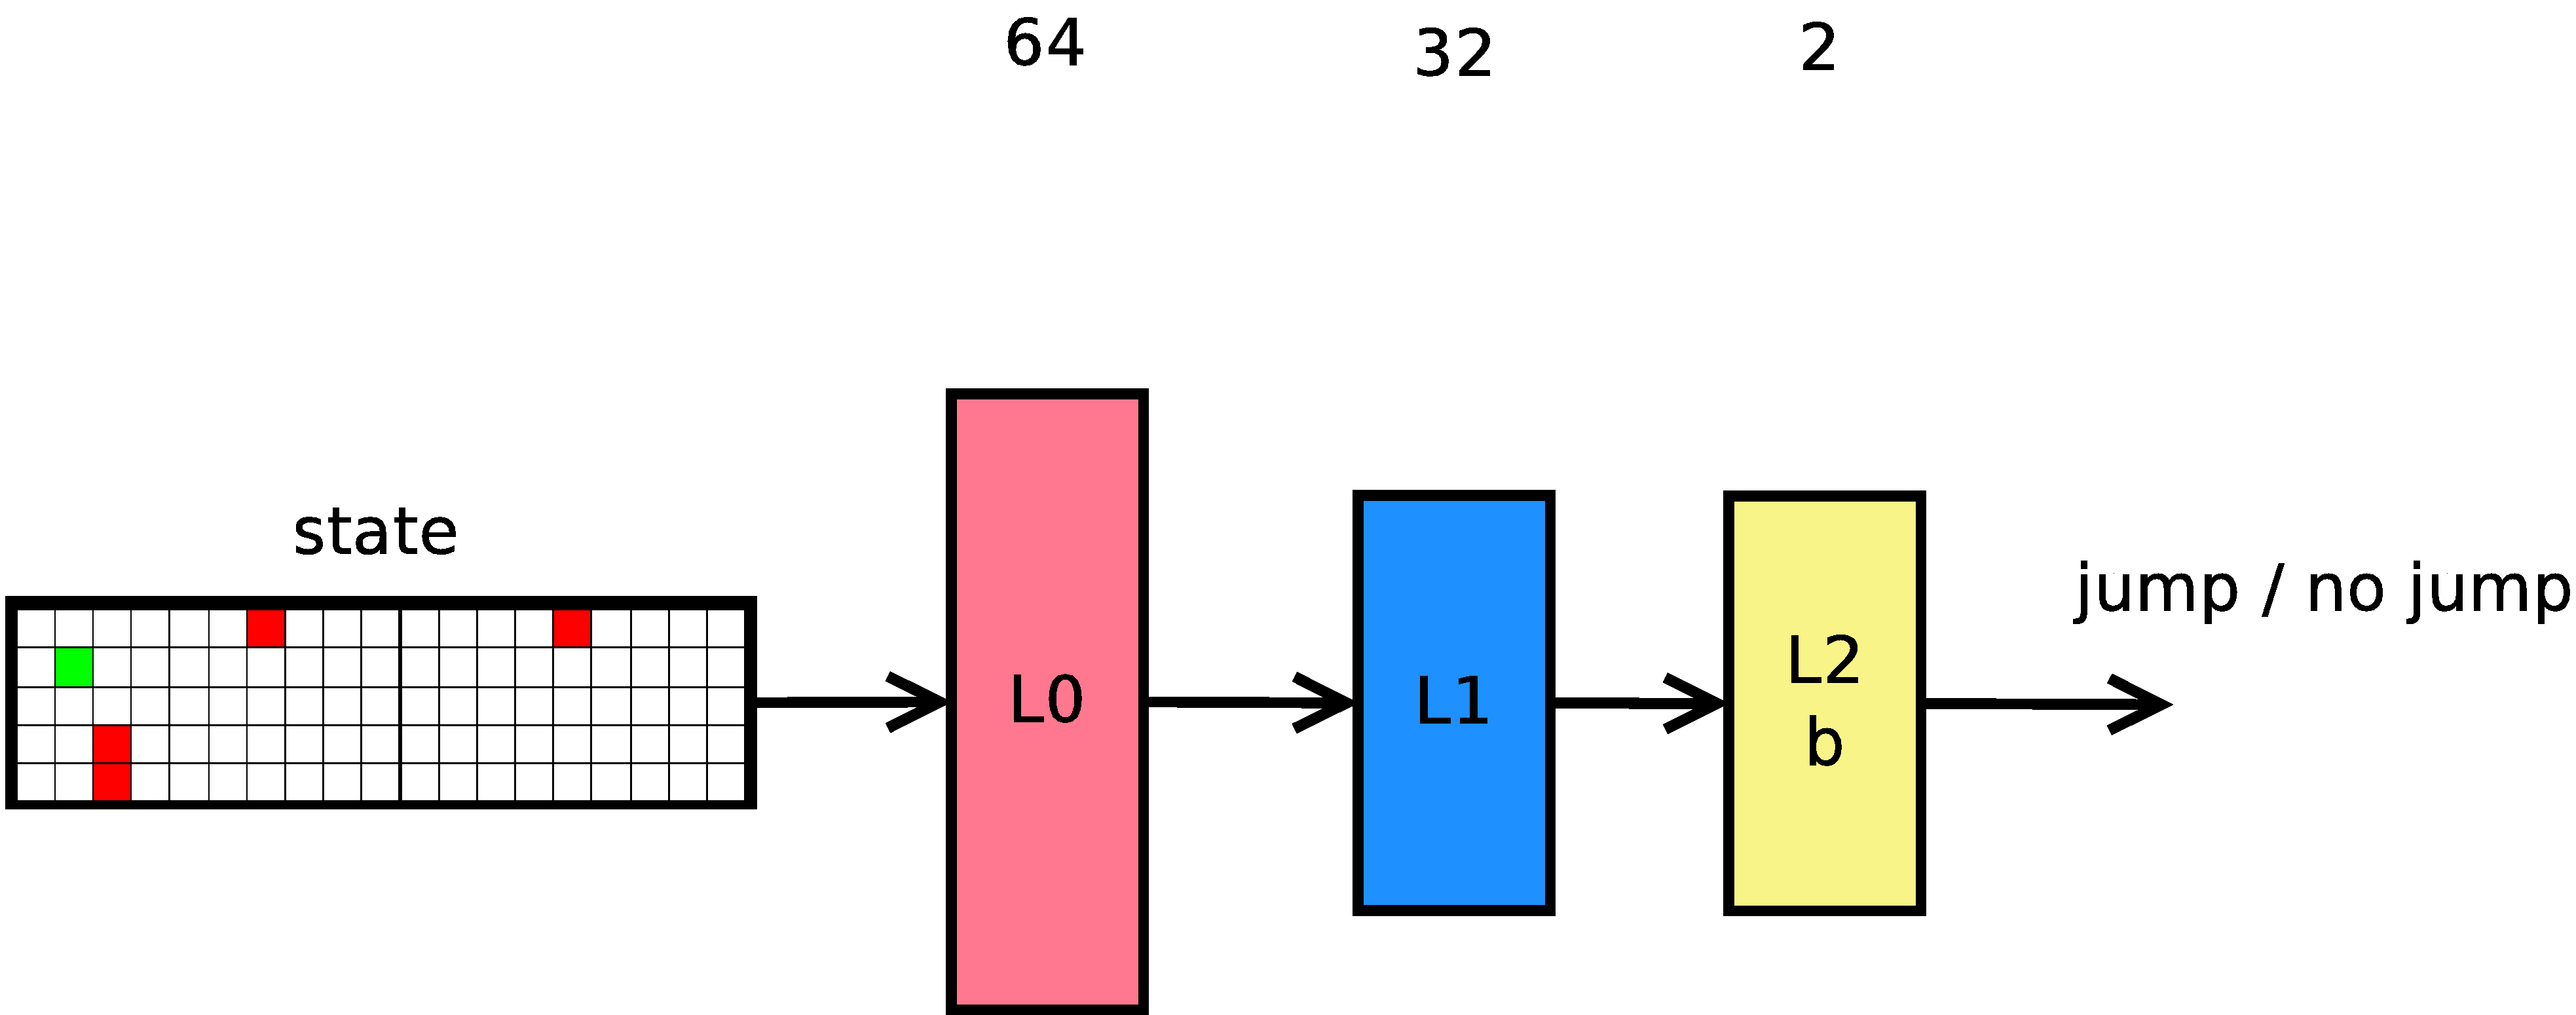
\includegraphics[scale=0.4]{../../diagrams/fnn.png}
  \caption{Supervised network architecture (FNN)}
  \label{img:Supervised network architecture}
\end{figure}


Druhá sieť je tvorená hlbokým autoenkóderom a doprednou sieťou (AE + FNN).
Skryté vrstvy majú aktivačnú funkciu ReLU, výstupná vrstva lineárnu aktivačnú funkciu.
Jej topológia je na obrázku \ref{img:Unsupervised + Supervised network architecture}.
Vo fáze unsupervised sa trénuje autoenkóder - z 95 prvkového vstupu, postupne extrahuje
príznaky, až na počet 32. Následne ďalšie dve vrstvy urobia rekonštrukciu vstupu.
Ako učenie sme zovlili metódu stacked autoencoder {\bf TODO citovat}: \\
najskôr sa urobí bypass medzi L1 a L2 vrstvami a trénujú sa len vrstvy L0 a L3,
po zvolenom počte itererácií sa pripoja vrstvy L1 a L2 a autoenkóder sa dotrénuje.
\\
Po natrénovaní autoenkódera sa odpoja vrstvy L2 a L3. Pripojením vrstvy L2b sa sieť
už trénuje supervised, podľa rovnice \ref{eq:rl_sarsa_learning}.

\begin{figure}[!h]
  \centering
  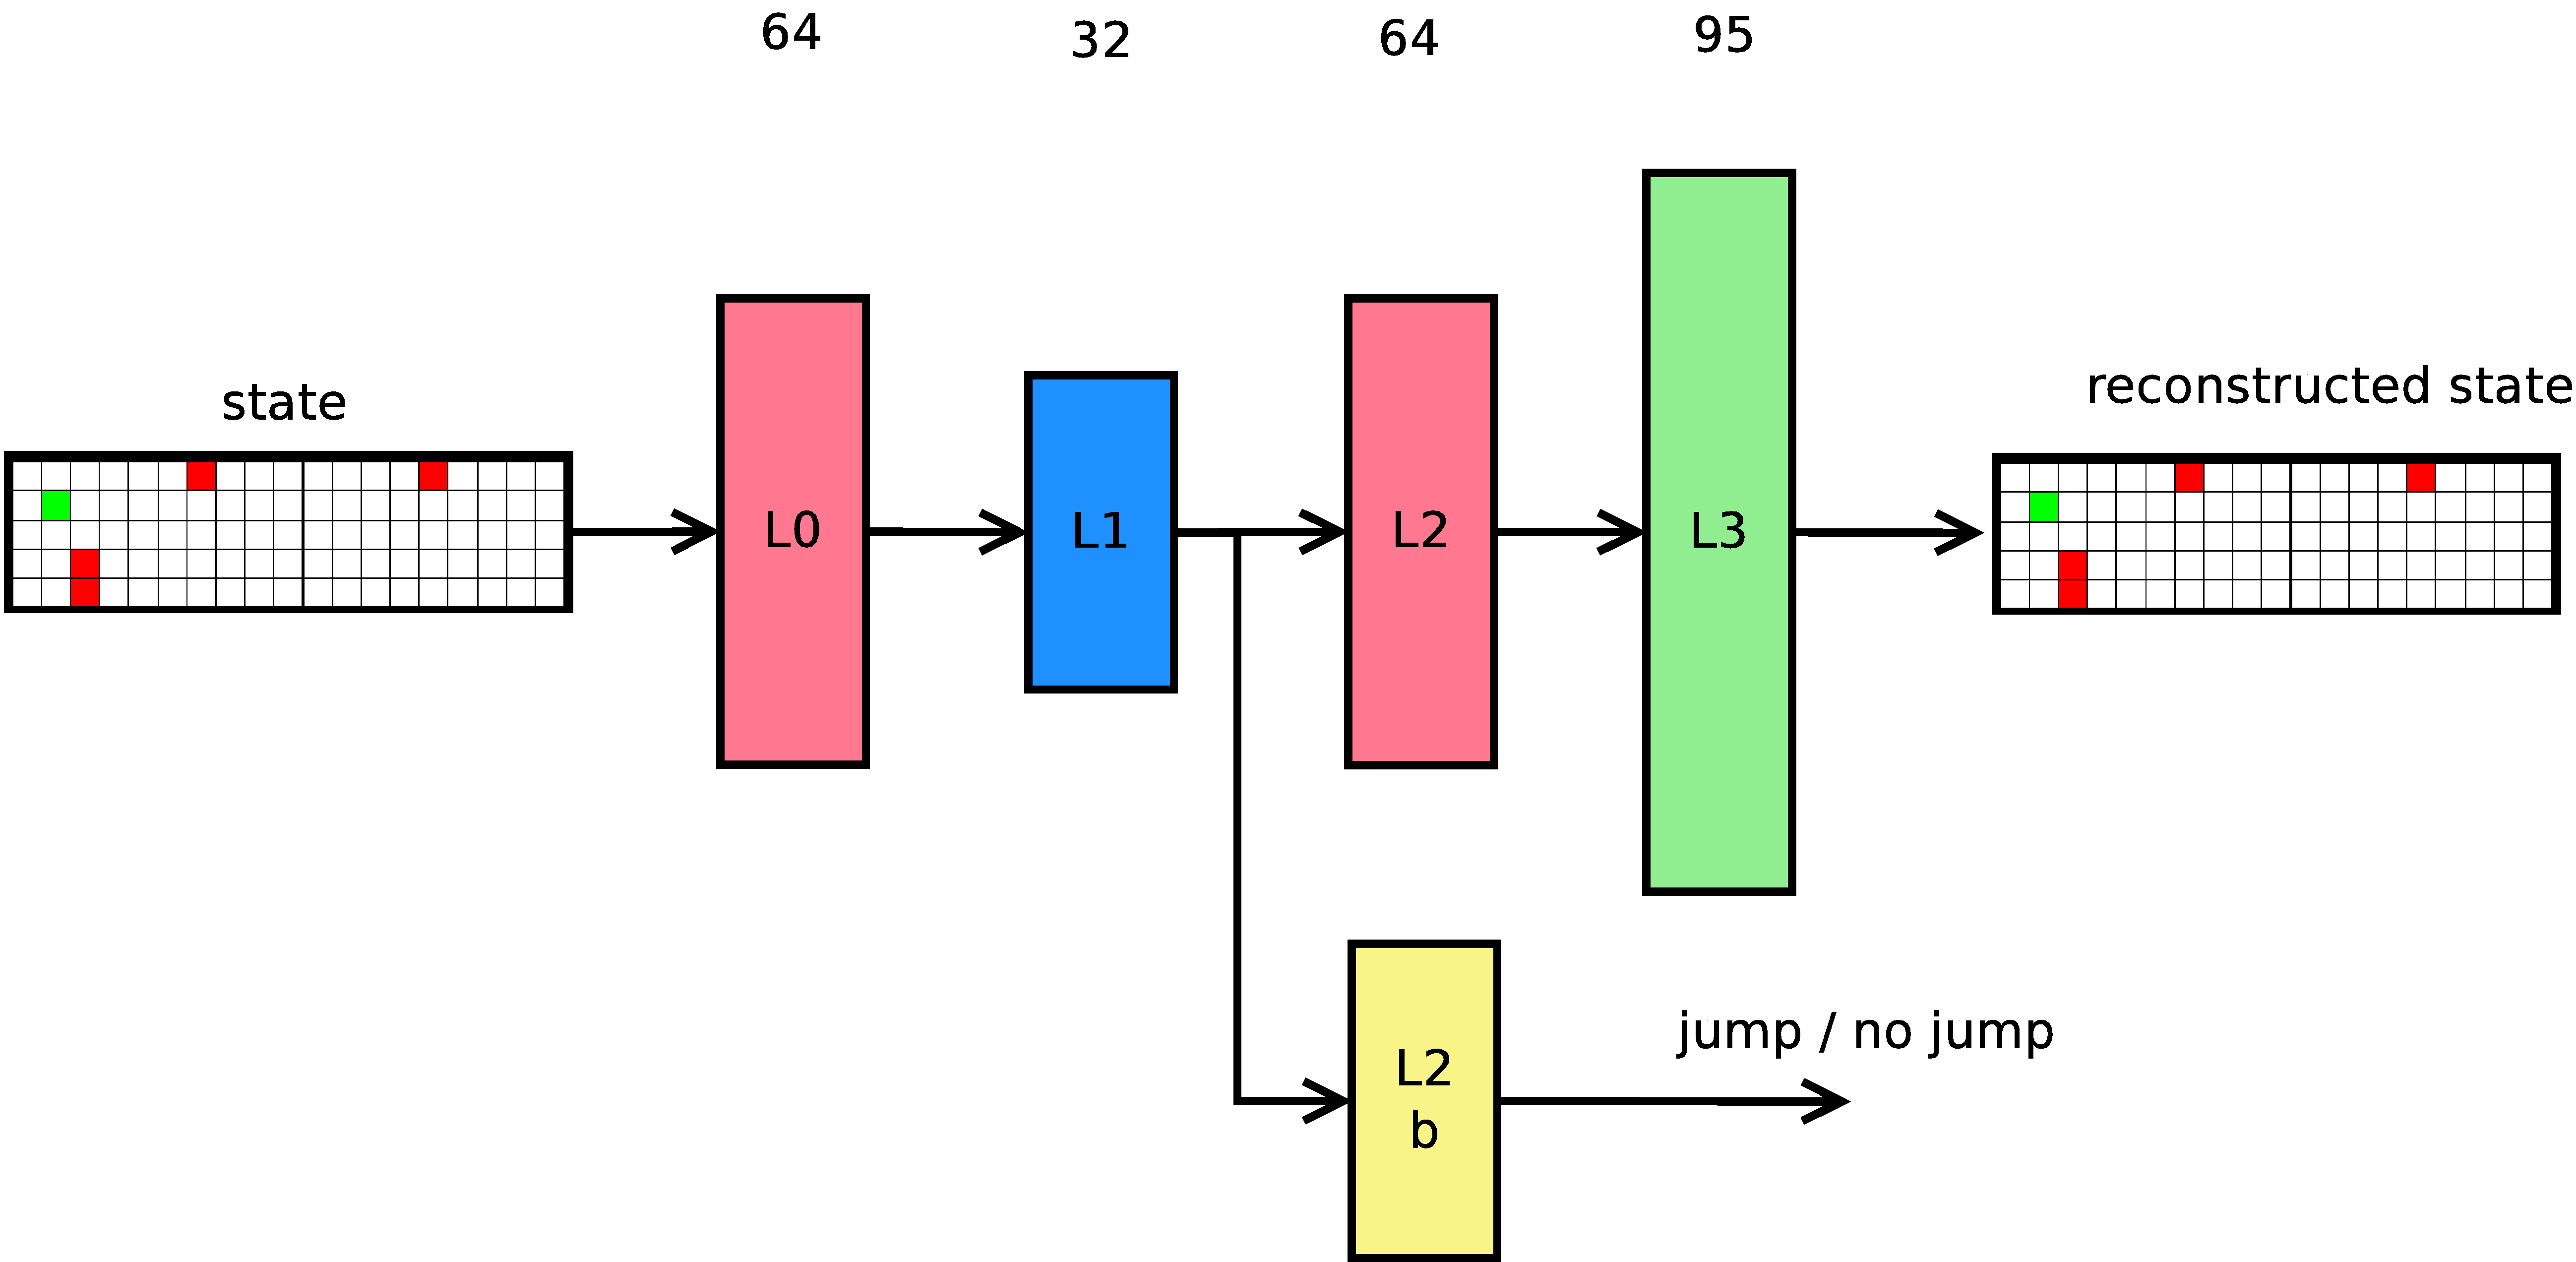
\includegraphics[scale=0.4]{../../diagrams/hnn.png}
  \caption{Unsupervised + Supervised network architecture (AE+FNN)}
  \label{img:Unsupervised + Supervised network architecture}
\end{figure}

\subsection{Parametre experimentu}

Experiment má mnoho parametrov, a bolo potrebné ich zafixovať - dnes nie
je možné analyticky stanoviť ich optimálne hodnoty.
Hyperparametre sietí boli experimentálne zvolené tak aby nedochádzalo k
divergencií váh. Úmerne tomu boli upravené počty iterácií učenia.
\\
Veľkosť batch bol zvolený na 1000 po sebe idúcich stavov. Každý batch mal pri tréningu
10 behov (epoch). Parameter SARSA algoritmu $\gamma$ bol zvolený $0.8$,
parameter $\alpha$ je pri použití neurónovej siete ukrytý v learning rate parametry siete.
Zvolená bola $\epsilon$ greedy stratégia voľby akcií. Voľba horšej akcie bola počas tréningu
0.1, počas testovania 0.0 - vyberala sa len najlepšia akcia.
\\
Siete boli učené algoritmom backpropagation. Riedkosť váh sa dosahovala pomocou L1 normy.
Gradientová metóda učenia váh potom prejde na vzťah

\begin{equation}
  \label{eq:weights_training}
  \Delta w = \eta E x \frac{df(y)}{dw} - \lambda sgn(w)
\end{equation}

kde \\
$E$ je chyba neurónu, \\
$x$ je vstup do neurónu, \\
$y$ je výstup neurónu, \\
$f$ je aktivačná funkcia, \\
$\eta$ je learning rate , \\
$\lambda$ je parameter riedkosti váh.

Hyperparametre siete sú zhrnuté v tabuľke \ref{tab:Hyperparametre siete}.

\begin{table}[!h]
\centering
\caption{Hyperparametre siete}
\label{tab:Hyperparametre siete}
\begin{tabular}{|l|l|l|l|l|}
\hline
                        & FNN sparse & FNN no sparse & AE+FNN  sparse & AE+FNN no sparse \\ \hline
unsupervised iterations & 0          & 0             & 100000         & 100000           \\ \hline
supervised iterations   & 200000     & 200000        & 200000         & 200000           \\ \hline
iterations per slice    & 0          & 0             & 50000          & 50000            \\ \hline
learning rate           & 0.0005     & 0.0005        & 0.0005         & 0.0005           \\ \hline
init weight range       & 0.1        & 0.1           & 0.1            & 0.1              \\ \hline
dropout                 & 0          & 0             & 0              & 0                \\ \hline
lambda                  & 0.00000001 & 0             & 0.00000001     & 0                \\ \hline
\end{tabular}
\end{table}

Menili sa parametre {\bf unsupervised iterations}, {\bf iterations per slice} a {\bf lambda}.
Parameter iterations per slice je počet iterácií na jednu úroveň stacked autoenkódera.

Sputené boli teda 4 rôzne experimenty, každý 5 krát, aby sa vylúčil vplyv počiatočných hodnôt váh
a dosiahol sa štatický vierohodný výsledok.


\section{Výsledky experimentov}

\subsection{Riedkosť váh}

Počas tréningu sa postupne váhy ustália na potrebné hodnoty. Pomocou histogramov
je možné overiť riedkosť váh, v závislosti od parametra $\lambda$.
Pre prehľadnosť sú znázornené len vlastnosti váh pre prvú vrstvu siete.
Histogramy na obrázkoch \ref{img:FNN sparse weights histogram} a \ref{img:FNN no sparse weights histogram}
porovnávajú početnosti váh pre doprednú sieť. Pre riedku sieť je 16\% váh nulových,
pre neriedku 1.67\%.
Podobné výsledky sú pre kombináciu autoenkódera a doprednej siete -
obrázky \ref{img:AE+FNN sparse weights histogram} a \ref{img:AE+FNN no sparse weights histogram}
S percentuálnym zastúpením 17.7\% pre riedke váhy a 3.3\% pre neriedke váhy.
Ilustračne ešte uvádzame cahrakter riedkych váh pre každý zo 64 neurónov, usporiadaných
do matice 5x19 - tak aby zodpovedali vizuálnej interpretácií prostredia. Obrázky
\ref{img:FNN sparse weights visualisation}, \ref{img:AE+FNN sparse weights visualisation}.


\begin{figure}[!htb]
\centering
\begin{minipage}{.5\textwidth}
  \centering
  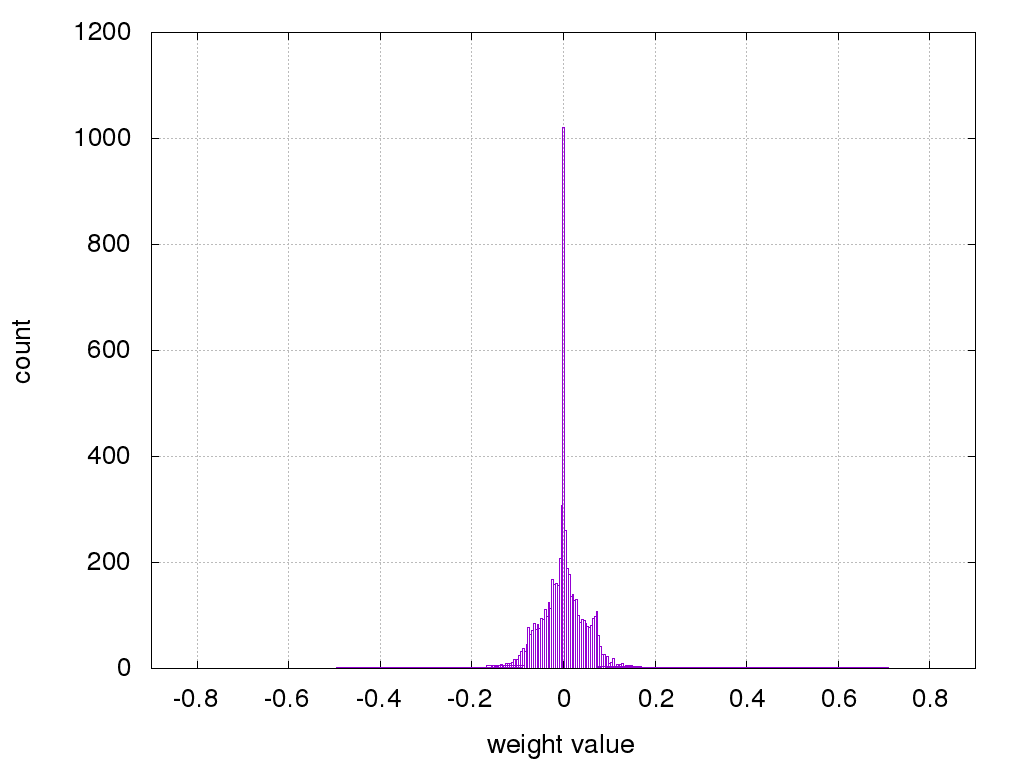
\includegraphics[scale=0.32]{../../results/rl_arcade/fnn_trained_0/supervised/layer_1_histogram.png}
  \captionof{figure}{FNN sparse weights histogram}
  \label{img:FNN sparse weights histogram}
\end{minipage}%
\begin{minipage}{.5\textwidth}
  \centering
  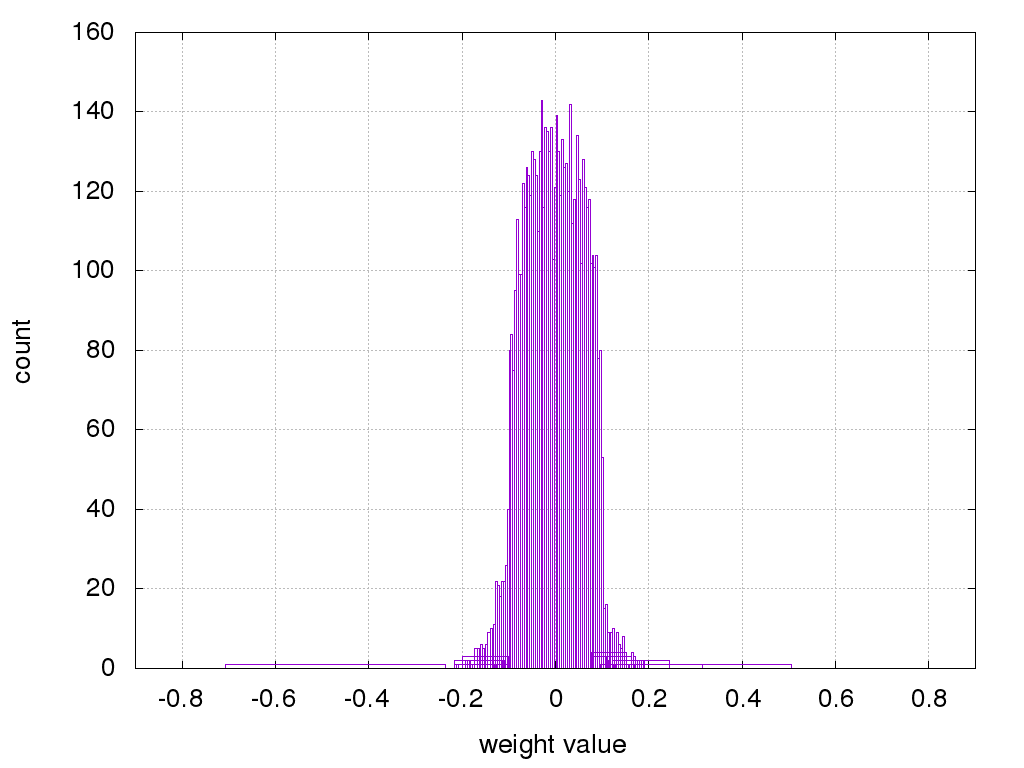
\includegraphics[scale=0.32]{../../results/rl_arcade/fnn_trained_5/supervised/layer_1_histogram.png}
  \captionof{figure}{FNN no sparse weights histogram}
  \label{img:FNN no sparse weights histogram}
\end{minipage}
\end{figure}

\begin{figure}[!htb]
\centering
\begin{minipage}{.5\textwidth}
  \centering
  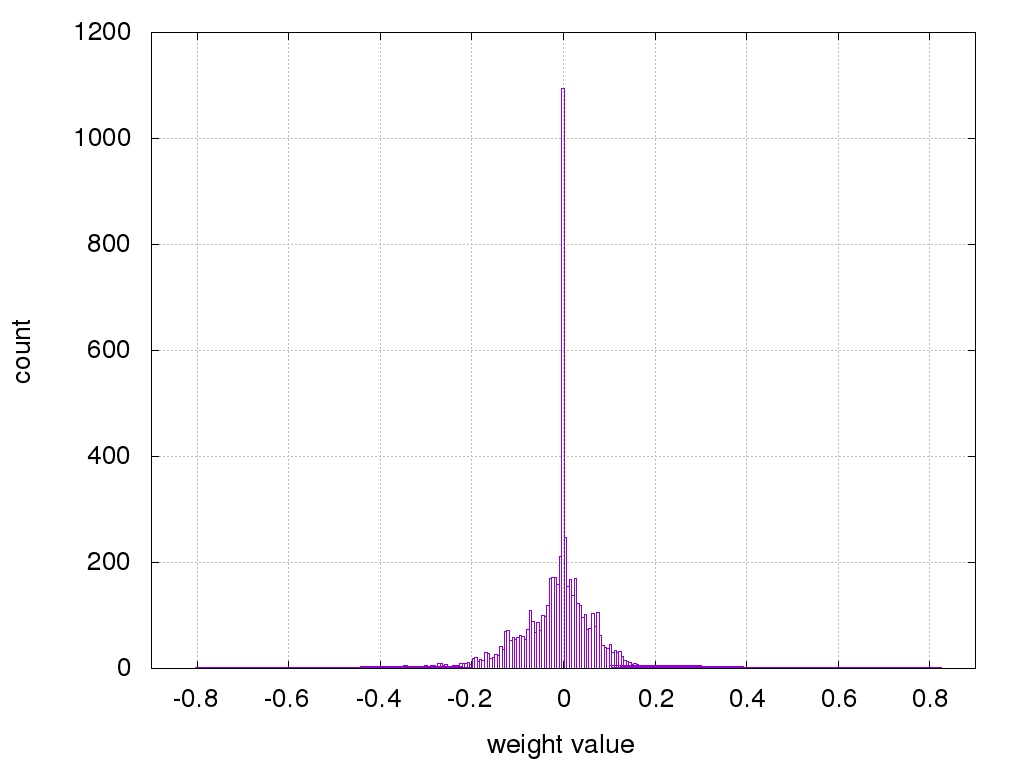
\includegraphics[scale=0.32]{../../results/rl_arcade/hnn_trained_0/supervised/layer_1_histogram.png}
  \captionof{figure}{AE+FNN sparse weights histogram}
  \label{img:AE+FNN sparse weights histogram}
\end{minipage}%
\begin{minipage}{.5\textwidth}
  \centering
  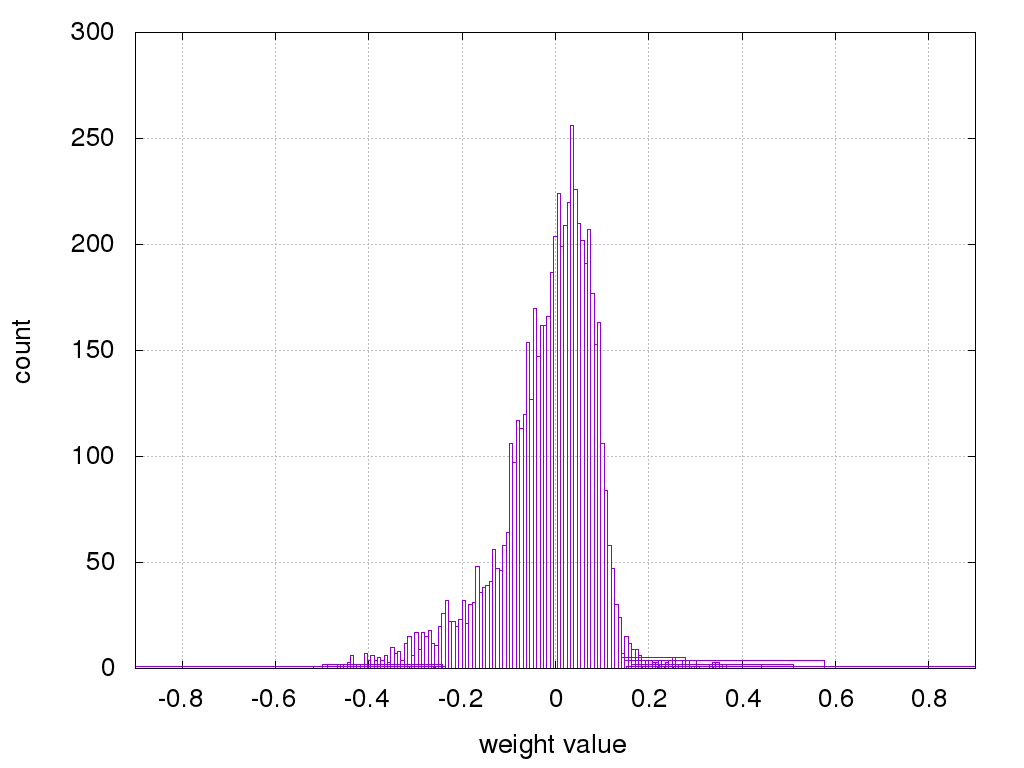
\includegraphics[scale=0.32]{../../results/rl_arcade/hnn_trained_5/supervised/layer_1_histogram.png}
  \captionof{figure}{AE+FNN no sparse weights histogram}
  \label{img:AE+FNN no sparse weights histogram}
\end{minipage}
\end{figure}



\begin{figure}[!htb]
\centering
\begin{minipage}{.5\textwidth}
  \centering
  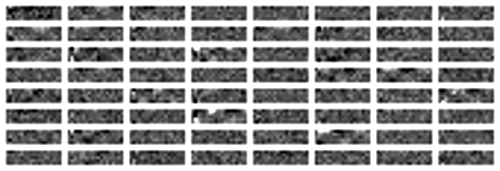
\includegraphics[scale=0.4]{../../diagrams/layer_1_fnn_sparse.png}
  \captionof{figure}{FNN sparse weights visualisation}
  \label{img:FNN sparse weights visualisation}
\end{minipage}%
\begin{minipage}{.5\textwidth}
  \centering
  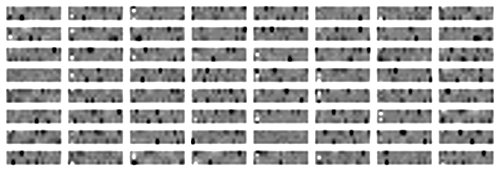
\includegraphics[scale=0.4]{../../diagrams/layer_1_hnn_sparse.png}
  \captionof{figure}{AE+FNN sparse weights visualisation}
  \label{img:AE+FNN sparse weights visualisation}
\end{minipage}
\end{figure}



\subsection{Dosiahnuté skóre}
Siet s autoenkóderom sa najpr predtrénovala 100 000 iteráciami. Následne sa spustil
supervised tréning. Po 200 000 supervised učiacich iteráciach sa spustilo 50 000 testovacích iterácií.
Zhrnuté dosiahnuté skóre na konci testovacích iteráciach je uvedené v tabuľke \ref{tab:summary_results}.


\begin{table}[]
\centering
\caption{Summary results}
\label{tab:summary_results}
\begin{tabular}{|l|c|c|c|c|}
\hline
                         & \multicolumn{1}{l|}{average score} & \multicolumn{1}{l|}{best score} & \multicolumn{1}{l|}{worst score} & \multicolumn{1}{l|}{average best action probability {[}\%{]}} \\ \hline
FNN sparse weights       & 960.58                             & 994.97                          & 922.64                           & 95.32                                                         \\ \hline
FNN nosparse weights     & 945.04                             & 995.64                          & 878.31                           & 93.29                                                         \\ \hline
AE+FNN sparse weights    & 914.5                              & 947.64                          & 875.31                           & 93.4                                                          \\ \hline
AE+FNN no sparse weights & 908.58                             & 954.31                          & 780.32                           & 93.12                                                         \\ \hline
\end{tabular}
\end{table}

Testovanie hypotézy o rýchlosti učenia zobrazujú grafy na obrázkoch
\ref{img:FNN progress comparison}, \ref{img:AE+FNN progress comparison}, \ref{img:Training progress comparison}.
Grafy zobrazujú priebehy pre všetkých 10 sieti (5 riedkych a 5 neriedkych).
Graf na obrázku \ref{img:FNN progress comparison} je pre jednoduchú doprednú sieť,
a graf na obrázku \ref{img:AE+FNN progress comparison} pre kombinvané riešenie s predtrénovaním.

Pre prehľadnosť sme z každého grafu vybrali 2 siete a vykreslili ich do spoločného grafu,
na obrázku \ref{img:Training progress comparison} - tento výber je možné urobiť, pretože rozptyly výsledkov sú
veľmi malé. Z grafu obrázka \ref{img:Training progress comparison} je zrejmé, že predtrénovaná
sieť sa učí rýchlejšie - voľbu správnej akcie dosiahne rýchlejšie.
Po čase podľa očakávania, obe siete dosiahnú rovnaký výsledok. Hypotéza sa teda potvrdila.

Rovnako nie je viditeľný kvalitatívny rozdiel medzi riedkymi a neriedkými váhami - optimalizáciou
harvéru na riedke výpočty by tak mohlo byť výrazne urýchlene.
Pre úplnosť dodávame dosiahnuté skóre počas testovania, obrázky
\ref{img:FNN score} a \ref{img:AE+FNN score}.
Po dostatočnom počte trénovacích iterácií sa teda všetky uvedené riešenia správajú veľmi
podobne.

\begin{figure}[!htb]
\centering
\begin{minipage}{.5\textwidth}
  \centering
  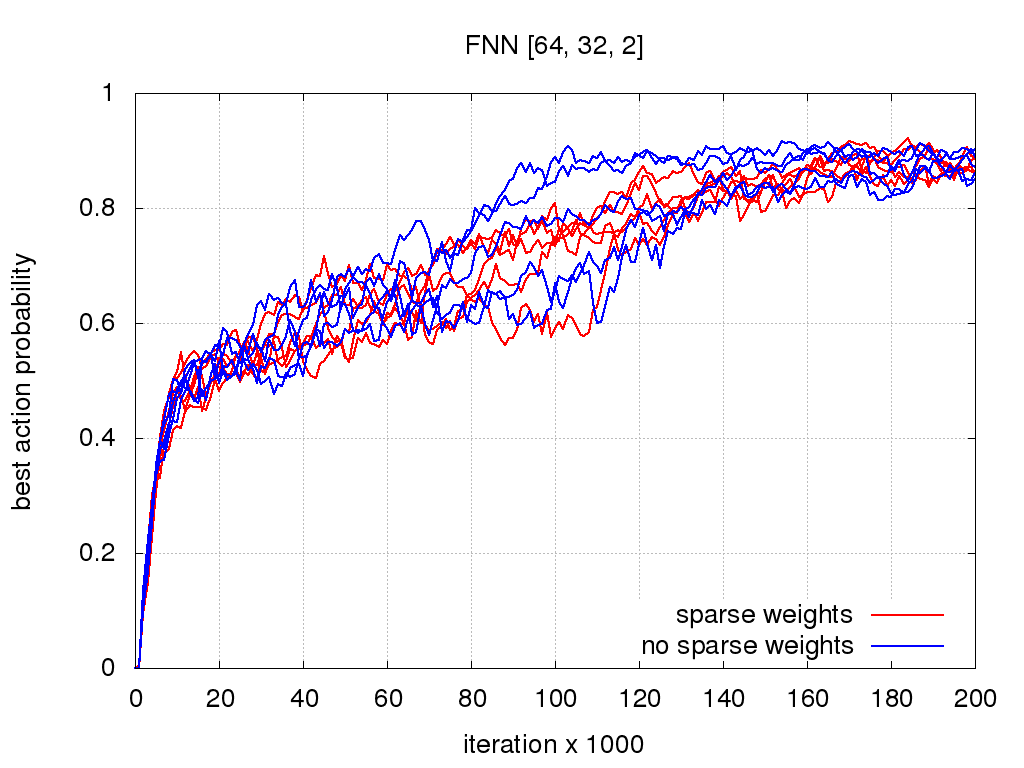
\includegraphics[scale=0.3]{../../results/rl_arcade/fnn_progress/training_progress.png}
  \captionof{figure}{FNN progress comparison}
  \label{img:FNN progress comparison}
\end{minipage}%
\begin{minipage}{.5\textwidth}
  \centering
  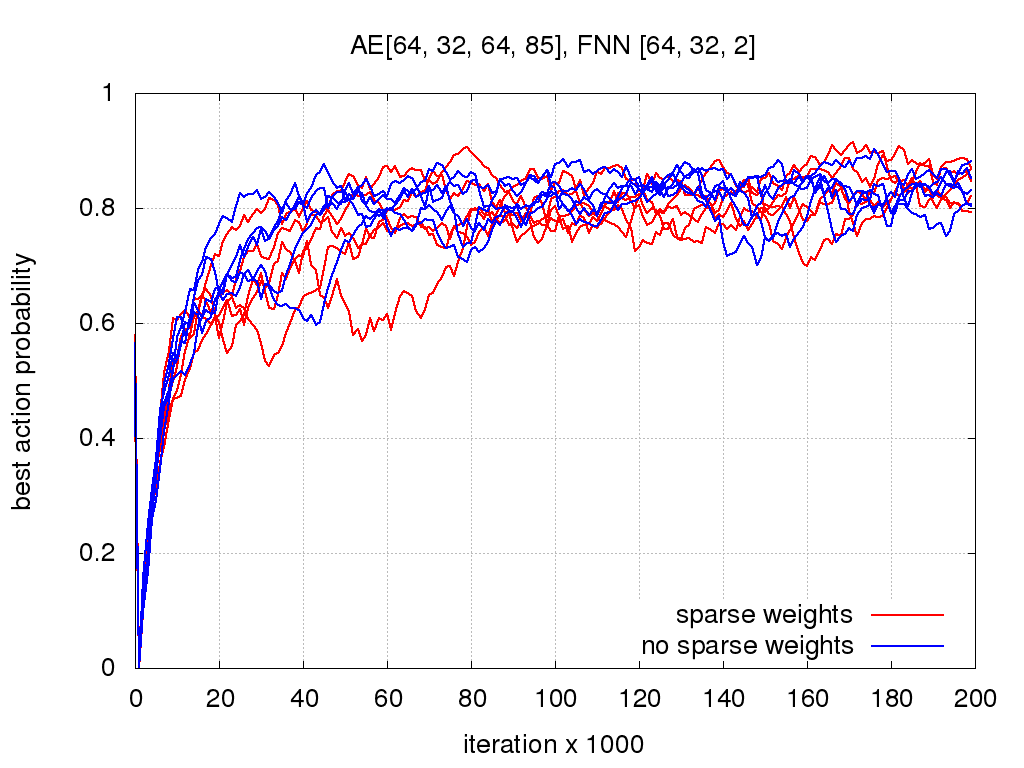
\includegraphics[scale=0.3]{../../results/rl_arcade/hnn_progress/training_progress.png}
  \captionof{figure}{AE+FNN progress comparison}
  \label{img:AE+FNN progress comparison}
\end{minipage}
\end{figure}




\begin{figure}[!htb]
\centering
\begin{minipage}{.5\textwidth}
  \centering
  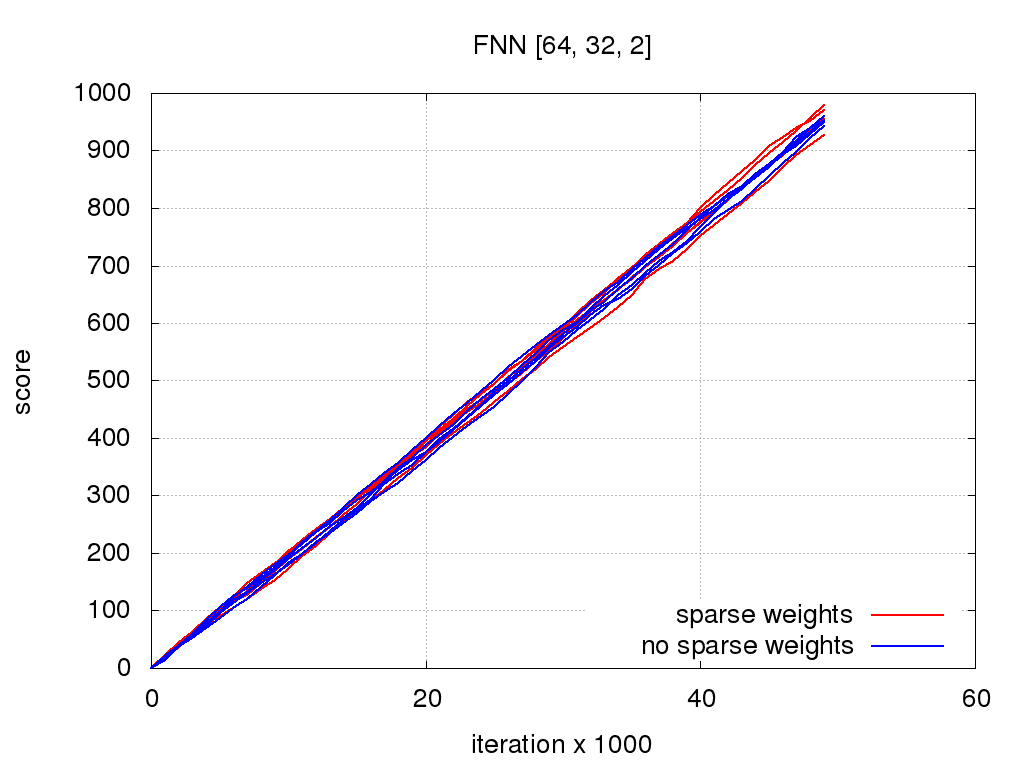
\includegraphics[scale=0.3]{../../results/rl_arcade/fnn_progress/testing_score.png}
  \captionof{figure}{FNN score}
  \label{img:FNN score}
\end{minipage}%
\begin{minipage}{.5\textwidth}
  \centering
  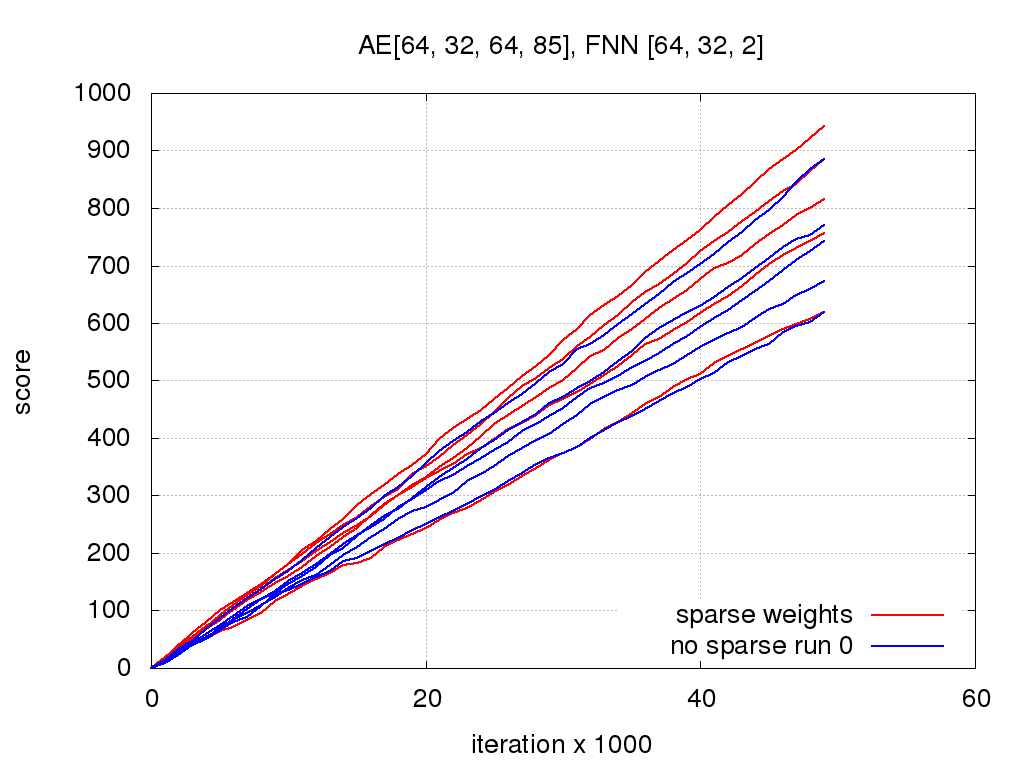
\includegraphics[scale=0.3]{../../results/rl_arcade/hnn_progress/testing_score.png}
  \captionof{figure}{AE+FNN score}
  \label{img:AE+FNN score}
\end{minipage}
\end{figure}






\begin{figure}[!h]
  \centering
  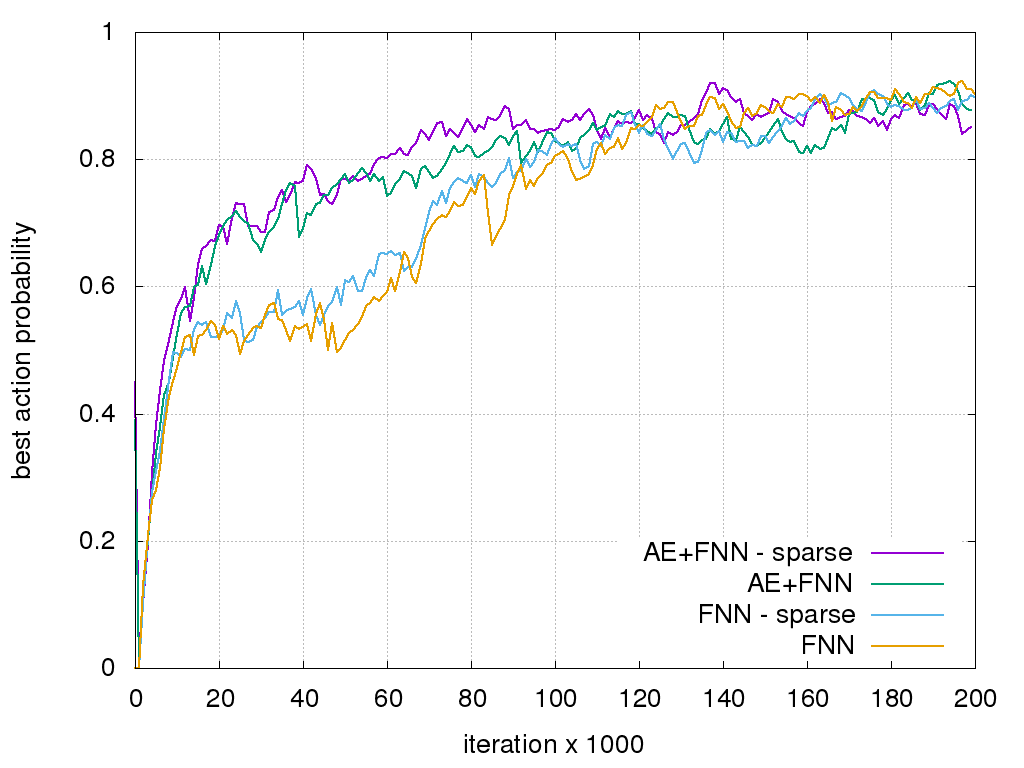
\includegraphics[scale=0.4]{../../results/rl_arcade/training_progress.png}
  \caption{Training progress comparison}
  \label{img:Training progress comparison}
\end{figure}



\newpage
\section{Aditional experiment - snake}

Pozitívne výsledky uvedeného experimentu nás viedli urobiť ešte jeden, doplnkový experiment.
Použili sme klasickú hru had - agent má za úlohu zbierať jedlo, obrázok \ref{img:Testing snake game}.
Za každé zjedenie je odmena $+0.1$, za vypadnutie z mapy $-1.0$. Agent - had, má na
hlave 32 senzorov, ktoré ho informujú o vzdialenosti k jedlu. Senzory sú rozmiestnené
v polkruhu, tak aby rovnomerne pokrývali zorné pole.
Agent má na výber tri akcie - vpred, vľavo, vpravo. Had je modelovaný ako diferenciálny
podvozok {\bf TODO citovat} so zotrvačnosťou. Uvedené akcie teda generujú dve sily, ktoré
menia polomer zatáčania, tak ako je uvedené na obrázku \ref{img:Agent schematics}.
Kolízie neboli v experimente použité.

Hyperparametre siete boli rovnaké ako v predošlom experimente.
Parametre agenta bolo nutné upraviť, pravdepodobnosť voľby horšej akcie $\epsilon = 0.3$,
veľkosť batch 100 krokov, a počet epoch batchu 10. S týmito parametrami sa bol agent schopný
učiť a za pomerne krátky čas dosahoval kladné odmeny.
Kedže úloha ma menej prvkový stavový vektor, zmenšili sme počty neurónov v sietiach.
Topológia autoenkódera bola 32, 8, 32, 32 a topológia doprednej siete
32 8 3 \footnote {pozri obrázky \ref{img:Supervised network architecture} a \ref{img:Unsupervised + Supervised network architecture}}.


\begin{figure}[!htb]
\centering
\begin{minipage}{.5\textwidth}
  \centering
  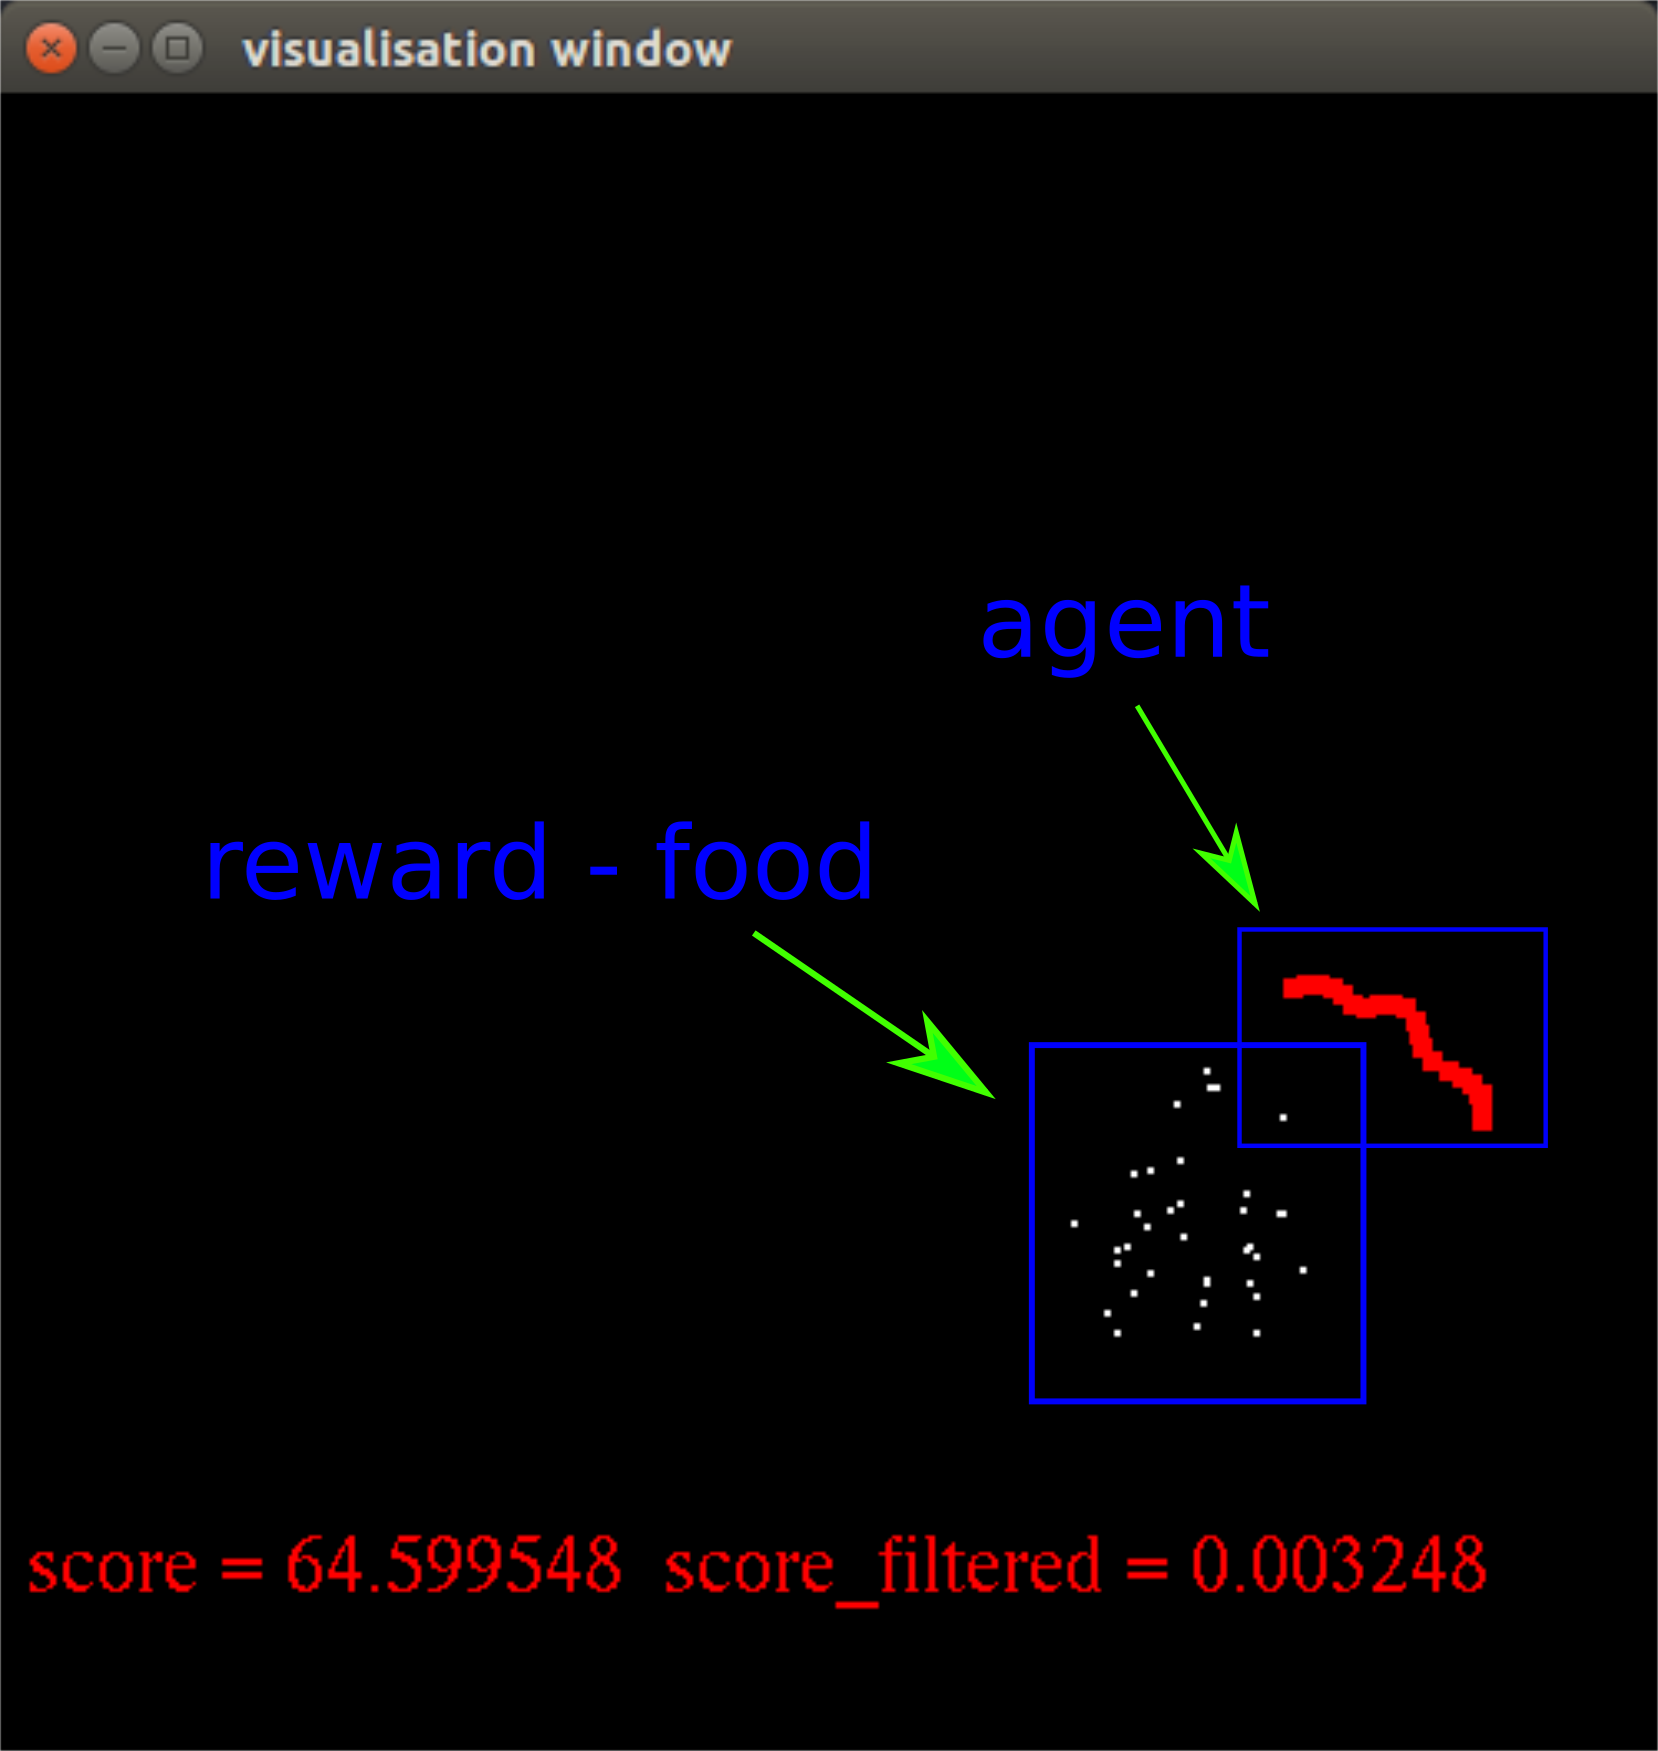
\includegraphics[scale=0.3]{../../diagrams/worms_rl_game_desc.png}
  \captionof{figure}{Testing snake game}
  \label{img:Testing snake game}
\end{minipage}%
\begin{minipage}{.5\textwidth}
  \centering
  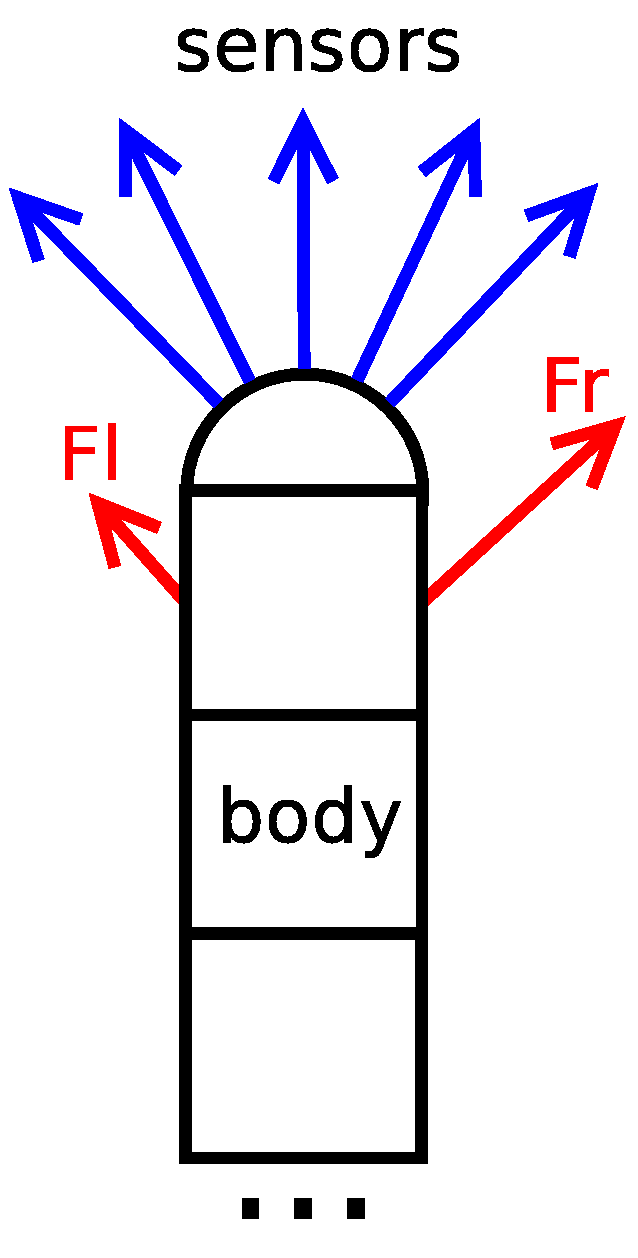
\includegraphics[scale=0.5]{../../diagrams/snake_bot_schem.png}
  \captionof{figure}{Agent schematics {\bf OBRAZOK je strasny}}
  \label{img:Agent schematics}
\end{minipage}
\end{figure}

\begin{figure}[!htb]
\centering
\begin{minipage}{.5\textwidth}
  \centering
  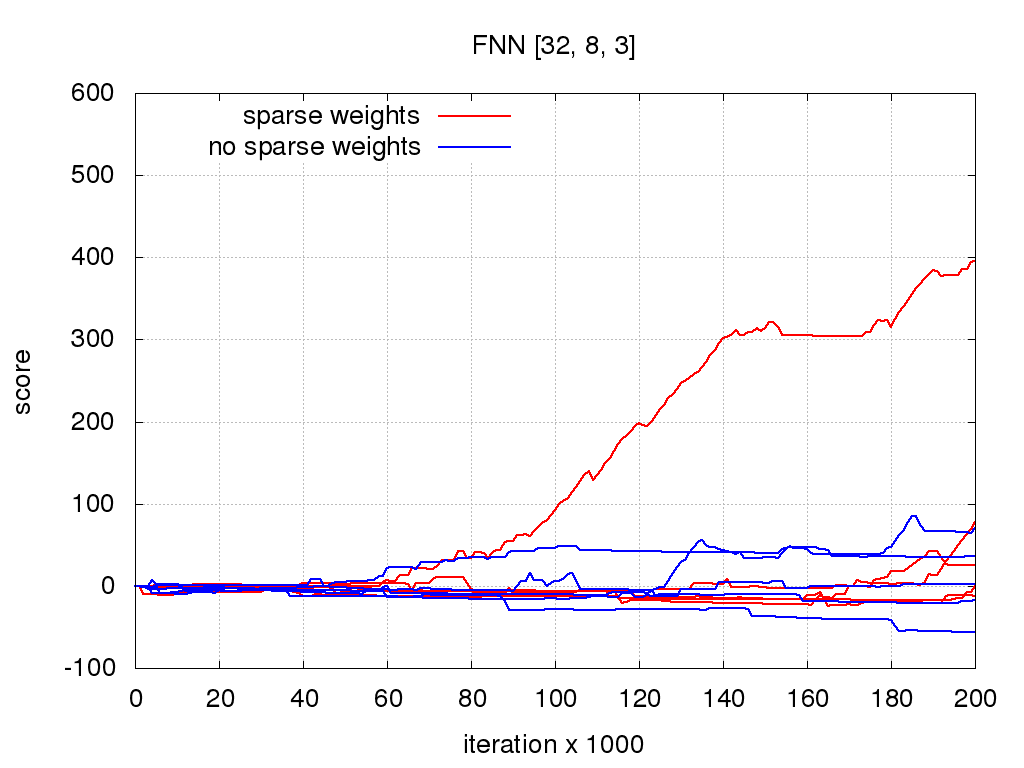
\includegraphics[scale=0.3]{../../results/rl_worms/fnn_progress/training_progress.png}
  \captionof{figure}{FNN score progress comparison}
  \label{img:worms FNN score progress comparison}
\end{minipage}%
\begin{minipage}{.5\textwidth}
  \centering
  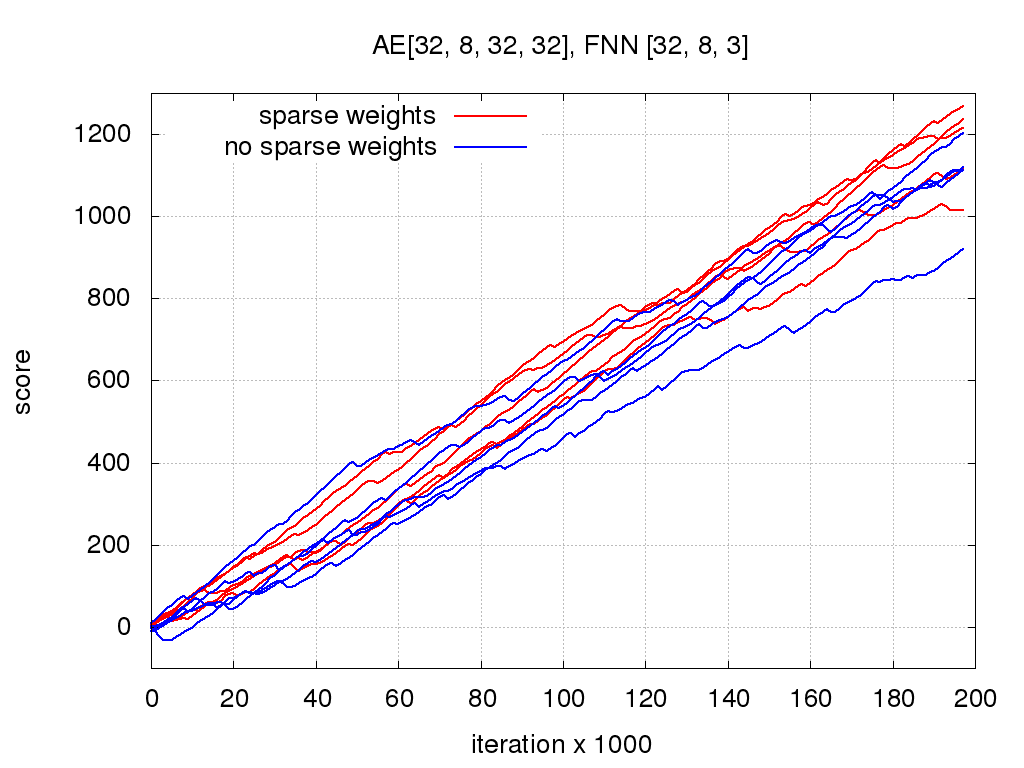
\includegraphics[scale=0.3]{../../results/rl_worms/hnn_progress/training_progress.png}
  \captionof{figure}{AE+FNN score progress comparison}
  \label{img:worms AE+FNN score progress comparison}
\end{minipage}
\end{figure}


\begin{figure}[!h]
  \centering
  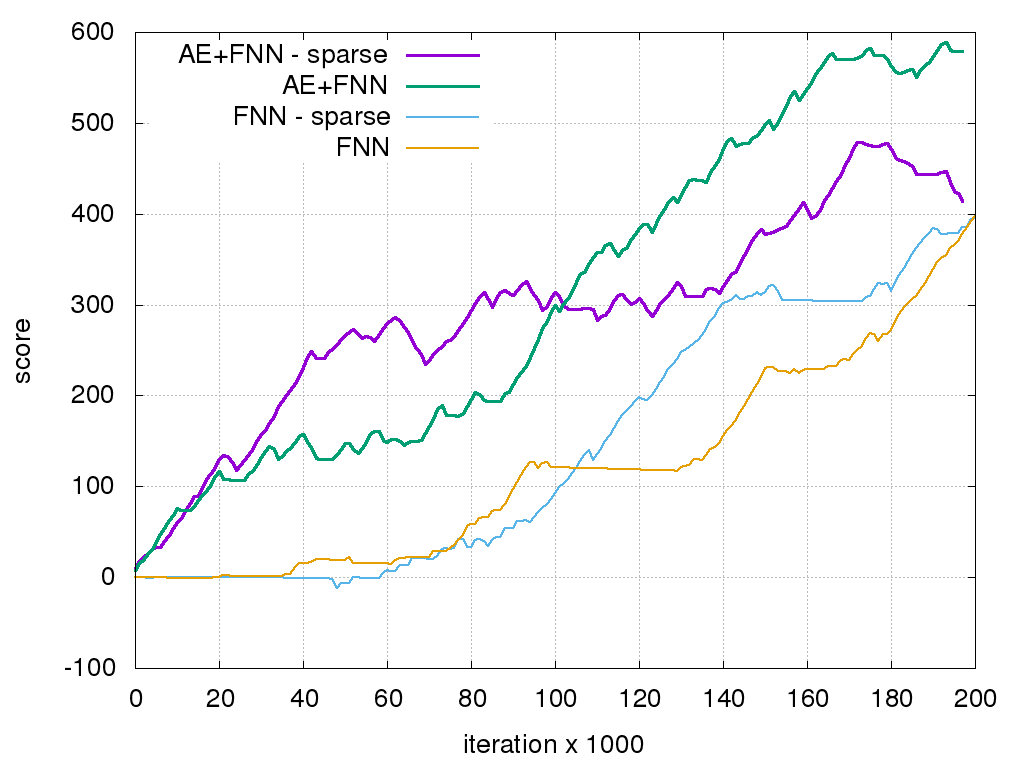
\includegraphics[scale=0.4]{../../results/rl_worms/training_progress.png}
  \caption{Training worms score progress for best networks}
  \label{img:Training worms score progress for best networks}
\end{figure}

Skóre dosiahnuté počas tréningu je na obrázkoch
\ref{img:worms FNN score progress comparison}, \ref{img:worms AE+FNN score progress comparison}
a   \ref{img:Training worms score progress for best networks}.
Vzhľadom na variabilitu výskytu odmien, sú ropztyly oveľa väčšie ako v predošlom experimente.
Prekvapujúce je zistenie, že niektoré dopredné siete nedosiahli kladné skóre ani po 200 000
trénovacií iteráciach. Naproti tomu, všetky predtrénované siete dosiahli kladné skóre,
tri z nich prekonali jednoduché dopredné siete. Na obrázku \ref{img:Training worms score progress for best networks}
sú znázornené najlepšie siete z oboch topológií pre porovnanie.
Naša hypotéza sa teda aj tu potvrdila - pretrénovanie siete naozaj zvýšilo rýchlosť
tréningu.




\newpage
\section{Conclusion}

Simulačný nástroj bol napísaný v C++, neurónové siete sú počítané pomocou NVIDIA Cuda
technológie. Je možné voliť medzi počítaním na CPU a GPU - výsledné zlepšenie závisí
od veľkosti siete. Beh experimentov bol asi 120 minút.

\newpage
\bibliographystyle{IEEEtran}
\bibliography{bib}

\begin{thebibliography}{4}

\bibitem{bib:sdm_01} M.J.Flynn, P.Kanerva, and N.Bhadkamkar, 1989, Sparse Distributed Memory: Principles and Operation
http://i.stanford.edu/pub/cstr/reports/csl/tr/89/400/CSL-TR-89-400.pdf

\bibitem{bib:sdm_02} David Rogers, 1988, NASA, KANERVA’S SPARSE DISTRIBUTED MEMORY: AN ASSOCIATIVE MEMORY ALGORITHM WELL SUITED TO THE CONNECTION MACHINE
https://pdfs.semanticscholar.org/9288/bb551f000348f800ff40d0fdb3fd74c410ef.pdf

\bibitem{bib:sdm_03} J. S. Albus, 1975, Data Storage in Cerebellar Model Articulation Controller
https://www.cs.cmu.edu/afs/cs/academic/class/15883-f13/readings/albus-1975.pdf



\bibitem{bib:sparse_01} Olshausen and Field (1997): Sparse coding with an overcomplete basis set
\bibitem{bib:sparse_02} Olshausen BA, Field DJ (2004) : Sparse coding of sensory inputs. Current Opinion in Neurobiology, 14, 481-487
\bibitem{bib:sparse_03} Mushroom body, locust  (Laurent)
\bibitem{bib:sparse_04} HVC, zebra finch (Fee)
\bibitem{bib:sparse_05} Auditory cortex, mouse  (DeWeese \& Zador)
\bibitem{bib:sparse_06} Hippocampus, rat\/primate(Thompson \& Best; Skaggs)
\bibitem{bib:sparse_07} Motor cortex, rabbit  (Swadlow)
\bibitem{bib:sparse_08} Visual cortex, monkey\/cat  (Vinje \& Gallant)
\bibitem{bib:sparse_09} Inferotemporal cortex, human (Fried \& Koch)



\end{thebibliography}

\end{document}
